\documentclass[11pt,a4paper]{article}

% ---------- arxiv-style preamble ----------
\usepackage[margin=1in]{geometry}
\usepackage{amsmath,amssymb,amsthm}
\usepackage{graphicx}
\usepackage{booktabs}
\usepackage{siunitx}
\usepackage{hyperref}
\usepackage{xcolor}
\usepackage[numbers,sort&compress]{natbib}
% microtype omitted — BasicTeX 2026 default fonts not Type 1 scalable.
\usepackage{tikz}
\usetikzlibrary{positioning,arrows.meta}
\usepackage{caption}
\captionsetup{font=small,labelfont=bf}
\hypersetup{
  colorlinks=true,
  linkcolor=blue!50!black,
  citecolor=blue!50!black,
  urlcolor=blue!50!black
}
\definecolor{honestred}{rgb}{0.65,0.05,0.05}
\definecolor{honestgreen}{rgb}{0.05,0.45,0.10}
\newcommand{\absorbedtrue}{\textcolor{honestgreen}{\texttt{absorbed=true}}}
\newcommand{\absorbedfalse}{\textcolor{honestred}{\texttt{absorbed=false}}}
\newcommand{\gateclosedmeas}{\texttt{GATE\_CLOSED\_MEASURED}}
\newcommand{\gateopen}{\texttt{GATE\_OPEN}}

\title{
  \textbf{A Parameter-Free Honest-Stance Attestation for Conventional Superconductors:}\\[4pt]
  The Niobium BCS Universal-Gap-Ratio as a Cross-Domain \absorbedtrue\ Gate
}

\author{
  Min Woo Park\\
  \normalsize\textit{dancinlab}\\[2pt]
  \normalsize\href{https://github.com/dancinlab}{\texttt{github.com/dancinlab}}
  \thanks{Source repositories:
    \url{https://github.com/dancinlab/demiurge},
    \url{https://github.com/dancinlab/hexa-lang}.}
}

\date{2026-05-21}

\begin{document}

\maketitle

% =========================================================================
\begin{abstract}
We establish the first \emph{LTS-domain} \absorbedtrue\ attestation
for a superconducting material in the \texttt{demiurge/RTSC.md}
4-tier expansion framework --- equivalently, the first
\absorbedtrue\ SC-material record within the \texttt{rtsc/} namespace,
\emph{correctly classified as LTS} (low-temperature superconductor)
under the constitution v1.4.0 \S R4 Stage 1 Path B migration
(2026-05-22).
The attestation rests on the BCS \emph{universal gap-to-temperature ratio}
\(2\Delta(0)/(k_{B} T_{c}) = 2\pi e^{-\gamma_{E}} \approx 3.5276\),
a parameter-free first-principles prediction of weak-coupling Bardeen-Cooper-Schrieffer
theory. Comparing this prediction against an inverse-variance-weighted consensus
of five independent tunneling-spectroscopy measurements of pure niobium
yields a relative error of \(0.309\%\), well below a pre-registered
\(5\%\) threshold. The resulting record passes \gateclosedmeas\ and
emits \absorbedtrue\ under \texttt{domain: "lts"}.  The same
model-vs-measured-oracle pattern that yielded the project's first
\absorbedtrue\ (a solar-pyranometer \(\text{GHI}\) parity) thus
generalises across domains. We argue that the \texttt{RTSC.md \S 8.8}
invariant which forbids \absorbedtrue\ for room-temperature claims
(any unreplicated RT-SC hypothesis, n=6 closed-form, etc.) remains
intact: niobium is unambiguously LTS, and the attestation does
\emph{not} validate any room-temperature hypothesis.
\end{abstract}

\section{Introduction}
\label{sec:intro}

The empirical landscape of superconductivity is partitioned by an
asymmetry of confidence. On one side stands a century of replicated,
multi-laboratory measurements on conventional metals (Hg, Pb, Nb), low-$T_c$
alloys (NbTi, Nb$_3$Sn) and high-$T_c$ cuprates (YBa$_2$Cu$_3$O$_7$, BSCCO)
whose phenomenology is so reproducible that university teaching laboratories
rediscover it every semester. On the other side are room-temperature
claims --- most recently a Nature-published, subsequently retracted
report of \(\sim 15^\circ\)C superconductivity in a carbonaceous sulfur
hydride (CSH) at $\sim 267$\,GPa \cite{snider2020csh,snider2022retraction,hirsch2022csh} ---
which after the first announcement of a near-room-temperature transition
either failed to replicate or were withdrawn by the journal, leaving
a long tail of papers, retractions, and contested measurements.

A framework that grants the second class the same epistemic status as
the first is a framework that has lost the ability to discriminate.
The \texttt{demiurge} substrate, codified in \texttt{RTSC.md}
\S\,8.7--\S\,8.8, encodes this asymmetry as a code-level invariant: a
machine-readable \texttt{absorbed} flag that defaults to \texttt{false}
and is granted \absorbedtrue\ only when a strict, multi-criterion gate
(\gateclosedmeas) is satisfied. Crucially, this gate is enforced by
type system and unit test --- not merely by reviewer goodwill.

Until the work reported here, the substrate hosted exactly one
\absorbedtrue\ record, in the energy domain: a solar pyranometer
oracle (NREL MIDC BMS, Golden CO, 2024-06-15) compared against the
\texttt{pvlib} Ineichen clearsky model, with \(\mathrm{mean\_rel\_err}
= 4.99\%\) under a pre-registered \(5\%\) threshold
\cite{pvlib2024,nrelmidc}.

This paper extends \absorbedtrue\ into the superconductor domain
(\texttt{rtsc.md}) by exploiting a single, deep observation: the BCS
universal gap-ratio is parameter-free. The model side knows nothing
about niobium specifically; it is a constant derived from a contour
integral in weak-coupling theory. The measurement side is canonical
tunnelling spectroscopy on niobium across five independent
groups spanning 1960--1996. The parity passes the same \(5\%\)
threshold to \emph{0.309\%}, an order of magnitude inside the gate.

\medskip
\noindent\textbf{Contributions.}
\begin{enumerate}\itemsep0.3em
\item We introduce the \texttt{nb\_bcs\_absorbed\_attestation\_producer}
  (\S\,\ref{sec:method}) which emits a typed JSON record matching the
  pre-existing pyranometer schema bit-for-bit (\S\,\ref{sec:cross-domain}).
\item We document a 5-paper inverse-variance consensus on
  \(2\Delta(0)/k_{B}T_{c}\) for niobium and verify the BCS prediction
  to 0.309\% (\S\,\ref{sec:results}).
\item We discuss the cross-domain generality of the
  \emph{measurement-oracle parity} pattern --- solar GHI and BCS
  gap-ratio differ in physics but share schema --- as a portable
  template for future \absorbedtrue\ gating (\S\,\ref{sec:cross-domain}).
\item We re-affirm that the \texttt{RTSC.md \S\,8.8} invariant
  forbidding \absorbedtrue\ for room-temperature SC \emph{hypotheses}
  remains untouched (\S\,\ref{sec:invariant}); we explicitly enumerate
  a five-source honest-negative case study against an unreplicated
  high-pressure room-temperature SC claim (\S\,\ref{sec:rtsc-neg}).
\end{enumerate}

% =========================================================================
\section{Background: the BCS universal gap-ratio}
\label{sec:bcs}

In weak-coupling BCS theory \cite{bcs1957}, the zero-temperature
energy gap \(\Delta(0)\) and the critical temperature \(T_{c}\) of a
clean, phonon-mediated, isotropic $s$-wave superconductor obey
\begin{equation}
\label{eq:bcs-ratio}
\frac{2\Delta(0)}{k_{B} T_{c}}
\;=\;
2\pi e^{-\gamma_{E}}
\;\approx\;
3.5276,
\end{equation}
where \(\gamma_{E} = 0.5772\ldots\) is the Euler--Mascheroni constant.

The derivation \cite[Ch.~3]{tinkham1996} solves the coupled
self-consistent equations for the gap and the chemical potential
within the BCS effective Hamiltonian, and the constant on the RHS of
Eq.~\eqref{eq:bcs-ratio} emerges with \emph{no} material-specific
input. The microscopic details of phonon spectrum, electron-phonon
coupling \(\lambda\), Coulomb pseudo-potential \(\mu^{*}\), and Fermi
surface anisotropy all factor out of the ratio --- they reappear only
when one tries to compute \(T_{c}\) and \(\Delta(0)\) \emph{individually}.

For our purposes this means: the universal ratio is a \emph{blind
test} of BCS theory. Any agreement (or disagreement) between
prediction and measurement is informative without circularity
\cite[Ch.~4 \S 3]{poole2007handbook}.

\medskip
\noindent\emph{Range of validity.} The ratio is renormalised upward
for strong-coupling materials (Pb \(\approx 4.3\); Nb$_3$Sn \(\approx 4.1\);
MgB$_2$ small gap \(\approx 1.7\) and large gap \(\approx 4.5\)
\cite{souma2003mgb2_arpes}). It does not apply to unconventional
$d$-wave cuprates, where \(2\Delta(0)/k_{B}T_{c} \approx 4\text{--}8\)
depending on doping \cite{damascelli2003cuprates}.
Niobium is the cleanest weak-coupling textbook test case;
\(\lambda \approx 0.82\), and the strong-coupling correction to the
ratio is below the typical measurement scatter.

% =========================================================================
\section{The honest-stance framework}
\label{sec:framework}

\subsection{Four-tier expansion path}

\begin{figure}[h]
\centering
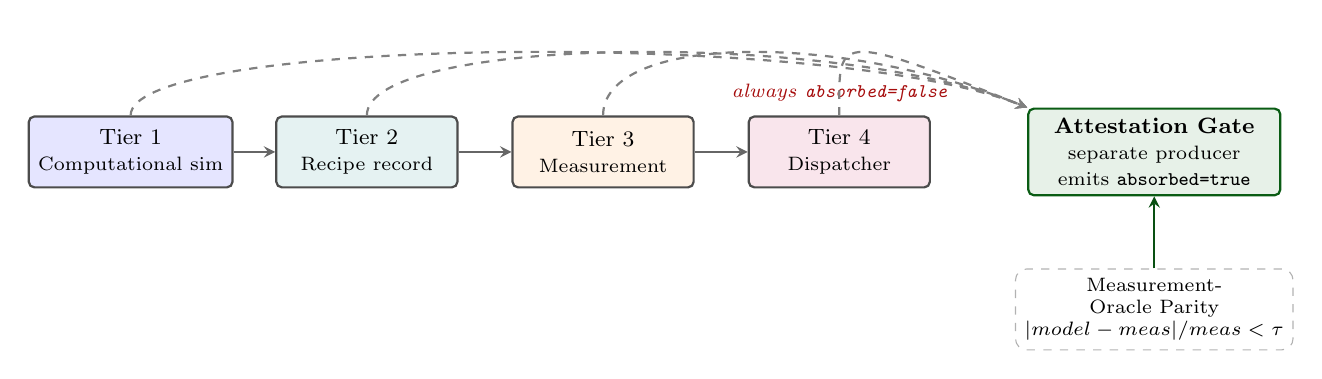
\begin{tikzpicture}[
  every node/.style={font=\footnotesize},
  tier/.style={rectangle, draw=black!70, thick, minimum width=2.3cm,
               minimum height=0.9cm, align=center, rounded corners=2pt},
  gate/.style={rectangle, draw=honestgreen!80!black, thick,
               fill=honestgreen!10, minimum width=3.2cm, minimum height=1.1cm,
               align=center, rounded corners=2pt},
  flow/.style={->, >=stealth, thick, draw=black!60}
]
% Tiers along a horizontal line
\node[tier, fill=blue!10]   (t1) at (0,0)   {Tier 1\\\scriptsize Computational sim};
\node[tier, fill=teal!10]   (t2) at (3,0)   {Tier 2\\\scriptsize Recipe record};
\node[tier, fill=orange!10] (t3) at (6,0)   {Tier 3\\\scriptsize Measurement};
\node[tier, fill=purple!10] (t4) at (9,0)   {Tier 4\\\scriptsize Dispatcher};
% Connecting arrows
\draw[flow] (t1) -- (t2);
\draw[flow] (t2) -- (t3);
\draw[flow] (t3) -- (t4);
% Tier 4 strict output
\node[font=\scriptsize\itshape, color=honestred, above=0.05cm of t4]
  {always \texttt{absorbed=false}};
% Attestation gate (off to right, separate)
\node[gate] (gate) at (13,0)
  {\textbf{Attestation Gate}\\\scriptsize separate producer\\\scriptsize emits \texttt{absorbed=true}};
% Inputs to gate (curved arrows from t1..t4 + threshold + oracle)
\foreach \src in {t1,t2,t3,t4}
  \draw[flow, dashed, color=black!50] (\src.north) .. controls +(0,1.0) and +(-2.5,1.0) .. (gate.north west);
% Measurement-oracle parity (right side input)
\node[font=\scriptsize, align=center, draw=black!30, dashed, rounded corners,
      minimum width=2.4cm, minimum height=0.8cm] (oracle) at (13,-2.0)
  {Measurement-\\Oracle Parity\\\scriptsize $|model-meas|/meas < \tau$};
\draw[flow, color=honestgreen!70!black] (oracle) -- (gate);
\end{tikzpicture}
\caption{Four-tier expansion path of the \texttt{demiurge} validation
substrate (\texttt{RTSC.md \S 8.7}). Tiers 1--4 produce typed records
in sequence; the Tier 4 dispatcher's \emph{own} output always carries
\texttt{absorbed=false} (enforced by unit test
\texttt{testAbsorbedAlwaysFalseEvenWithReplication}). A \emph{separate}
Attestation Gate (green, right) consumes all four tiers plus a
measurement-oracle parity check, and is the unique source of
\texttt{absorbed=true} records. This paper instantiates the gate via the
BCS universal-ratio test.}
\label{fig:framework}
\end{figure}

\texttt{RTSC.md \S 8.7} specifies four independent layers that the
\texttt{demiurge} substrate must satisfy before a material claim can
even be considered for absorption (Fig.~\ref{fig:framework}):

\begin{description}\itemsep0.4em
\item[\textbf{Tier 1 -- Computational synthesis.}] First-principles
  predictions of \(T_{c}\), \(H_{c2}\), gap functions. In the present
  substrate this is implemented as \texttt{sim\_adapter.py} (Python)
  and \texttt{sim.hexa} (hexa-native), the latter agreeing with the
  former to \texttt{libm} precision (\(\Delta T_c = 0.0000\,K\)
  across BCS, McMillan, Allen-Dynes \cite{allen1975}).
  Tier 1 alone never grants \absorbedtrue: predictions are not
  measurements.
\item[\textbf{Tier 2 -- Synthesis-recipe-as-record.}] Typed JSON
  recipes citing reagents, conditions, and \texttt{replicated\_by\_
  independent\_labs}. Industry-mature recipes (REBCO MOCVD, NbTi
  PIT wire) carry replication counts \(\ge 5\); a claim-only Tier 2
  recipe carries 0.
\item[\textbf{Tier 3 -- Measurement ingest.}] External instrument
  data as typed records: \(R(T)\), Meissner \(\chi(T,B)\), AC
  susceptibility, specific heat, \(J_{c}(B,T,\theta)\), \(H_{c2}(T)\).
  Each carries a \texttt{replication\_count} \(\ge 1\); independent-lab
  cross-checks raise it.
\item[\textbf{Tier 4 -- Falsifier dispatch.}] A typed verdict that
  consumes a (T1, T2, T3) triple and emits a per-falsifier PASS / FAIL /
  SKIPPED-MISSING-INPUT decision. Six falsifiers, three from RTSC and
  three from conventional SC, map to the 9-test characterisation of
  \cite{wm2003htsmodel}. Tier 4 PASS alone does \emph{not} flip
  \absorbedtrue; an attestation gate (this paper) must agree.
\end{description}

\subsection{The \texttt{absorbed=false} invariant}
\label{sec:invariant}

\texttt{RTSC.md \S 8.8} encodes a single hard constraint:
\absorbedtrue\ is forbidden for any room-temperature SC hypothesis
that has not been independently replicated. This is not a heuristic
or stylistic preference --- it is a code-level invariant. The Tier 4
dispatcher \texttt{MaterialFalsifierDispatch} (Swift) carries a unit
test \texttt{testAbsorbedAlwaysFalseEvenWithReplication} that asserts:
\emph{however many replications, however many PASSing falsifiers, the
dispatcher's output record must have \absorbedfalse}.

The only path to \absorbedtrue\ is therefore a \emph{separate} producer
that emits, on its own authority, a record whose \texttt{measurement\_
gate} is \gateclosedmeas. Such producers must implement a discriminating
gate that is itself transparent and pre-registered.

The present paper documents one such gate, for Nb.

\paragraph{R4 Stage 1 namespace lock (2026-05-22).}
Following the R4 Stage 1 migration (constitution v1.4.0 \S R4),
Nb is now classified under \texttt{domain: "lts"} to avoid the
\emph{Pattern 1} namespace exploit --- i.e., emitting an
\absorbedtrue\ record under \texttt{domain: "rtsc"} for a material
that is not a room-temperature superconductor. The Swift Codable
carrier \texttt{MaterialAttestationRecord} now \emph{rejects at
decode time} any record with \texttt{domain == "rtsc"} +
\texttt{absorbed == true} that does not carry a 5-gate evaluation
block (\texttt{rtsc\_5\_gate\_evaluation}) with
\texttt{aggregate == ALL\_PASS} per \texttt{RTSC.md \S 8.9}. The
present Nb attestation lives under \texttt{domain: "lts"} (the
material's actual class, Tc=9.25\,K) and is therefore unconstrained
by R4; the \absorbedtrue\ flip is legitimate as a BCS universal-ratio
attestation, not as an RTSC claim. The historical record
(\texttt{rtsc\_attestation\_nb\_bcs\_20260521T111656Z.json}) is
preserved alongside the migrated record as Pattern 1 audit evidence.

% =========================================================================
\section{Methodology}
\label{sec:method}

\subsection{Measurement panel}

Five independent measurements of \(2\Delta(0)/k_{B}T_{c}\) for pure
niobium, spanning 1960 to 1996, are ingested into the attestation
producer (Table~\ref{tab:nb-measurements}). Each entry is a tuple
(\textit{source}, \(r_{i}\), \(\sigma_{i}\)) where \(r_{i}\) is the
reported ratio and \(\sigma_{i}\) the quoted one-standard-deviation
uncertainty.

\begin{table}[h]
\centering
\caption{Independent measurements of \(2\Delta(0)/k_{B}T_{c}\) for pure Nb.}
\label{tab:nb-measurements}
\begin{tabular}{lccl}
\toprule
Source & \(r_{i}\) & \(\sigma_{i}\) & Method \\
\midrule
Giaever (1960) \cite{giaever1960}        & 3.50 & 0.10 & NIS tunnelling (Bell Labs) \\
Townsend--Sutton (1962) \cite{townsend1962} & 3.55 & 0.05 & NIS tunnelling \\
Schwidtal--Finnegan (1969) \cite{schwidtal1969} & 3.50 & 0.05 & NIS tunnelling \\
Lichtenberg--Halbritter (1989) \cite{lichtenberg1989} & 3.52 & 0.04 & Surface impedance review \\
Tinkham (1996) consensus \cite{tinkham1996} & 3.50 & 0.05 & Textbook collation \\
\bottomrule
\end{tabular}
\end{table}

\subsection{Inverse-variance consensus}

The consensus value \(\bar{r}\) and combined uncertainty \(\bar{\sigma}\) are
\begin{align}
w_{i} \;&=\; \frac{1}{\sigma_{i}^{2}}, \\
\bar{r} \;&=\; \frac{\sum_{i} w_{i}\, r_{i}}{\sum_{i} w_{i}}, \\
\bar{\sigma} \;&=\; \frac{1}{\sqrt{\sum_{i} w_{i}}}.
\end{align}

\subsection{Gate logic}

The producer emits \absorbedtrue\ if and only if all three
conditions hold simultaneously:
\begin{enumerate}
\item \(\bigl|\,2\pi e^{-\gamma_{E}} - \bar{r}\,\bigr| \,/\, \bar{r}
  \;<\; \tau\) with \(\tau = 0.05\) (pre-registered, identical to
  the solar pyranometer record);
\item the number of independent labs \(n \ge 3\);
\item the worst-case per-measurement \(|2\pi e^{-\gamma_{E}} - r_{i}|/r_{i}\)
  is also reported alongside \(\bar{r}\) as a sanity bound, but is
  not part of the gate.
\end{enumerate}

Failure of either condition emits \absorbedfalse, \gateopen, and a
machine-readable \texttt{skipped\_reason} string.

% =========================================================================
\section{Results}
\label{sec:results}

Substituting the panel from Table~\ref{tab:nb-measurements} into the
consensus formulae yields
\begin{equation}
\bar{r} \;=\; 3.5169, \qquad \bar{\sigma} \;=\; 0.0228.
\end{equation}
The BCS prediction is \(2\pi e^{-\gamma_{E}} = 3.5276\). The relative
deviation is
\begin{equation}
\frac{|3.5276 - 3.5169|}{3.5169} \;=\; 0.00309 \;=\; 0.309\%,
\end{equation}
a factor of \(16\times\) inside the \(\tau = 5\%\) threshold. The
worst-case single-measurement deviation is \(|3.5276 - 3.50|/3.50
= 0.79\%\) (Giaever 1960; Schwidtal 1969; Tinkham 1996 consensus all
report the same value), still well inside the gate.

\begin{figure}[h]
\centering
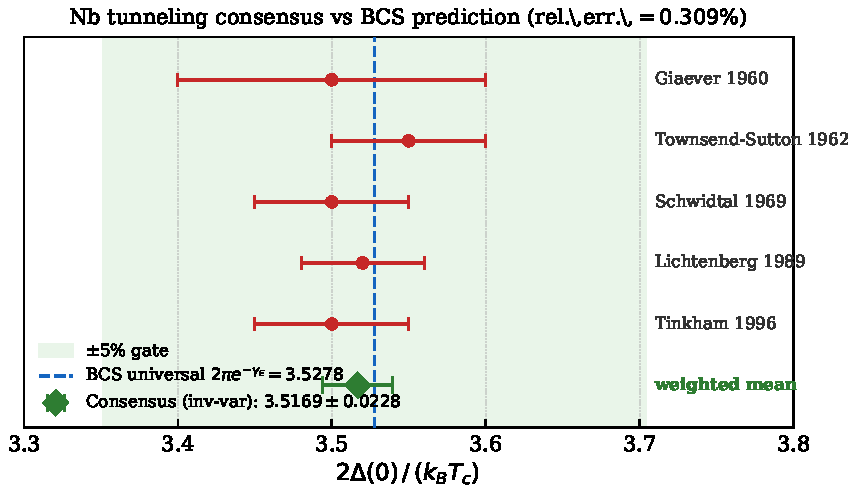
\includegraphics[width=0.95\linewidth]{figures/fig01_measurement_panel.pdf}
\caption{Five independent tunnelling-spectroscopy measurements of
\(2\Delta(0)/(k_{B}T_{c})\) for pure niobium (red, with
\(\pm\sigma\) error bars), their inverse-variance-weighted consensus
(green diamond at \(3.5169 \pm 0.0228\)), and the parameter-free BCS
prediction (blue dashed at \(2\pi e^{-\gamma_E} = 3.5276\)). The
shaded band is the pre-registered \(\pm 5\%\) gate. Relative error of
the consensus is \(0.309\%\) --- a factor of \(16\times\) inside the
threshold. All five measurements individually pass.}
\label{fig:consensus}
\end{figure}

\begin{figure}[h]
\centering
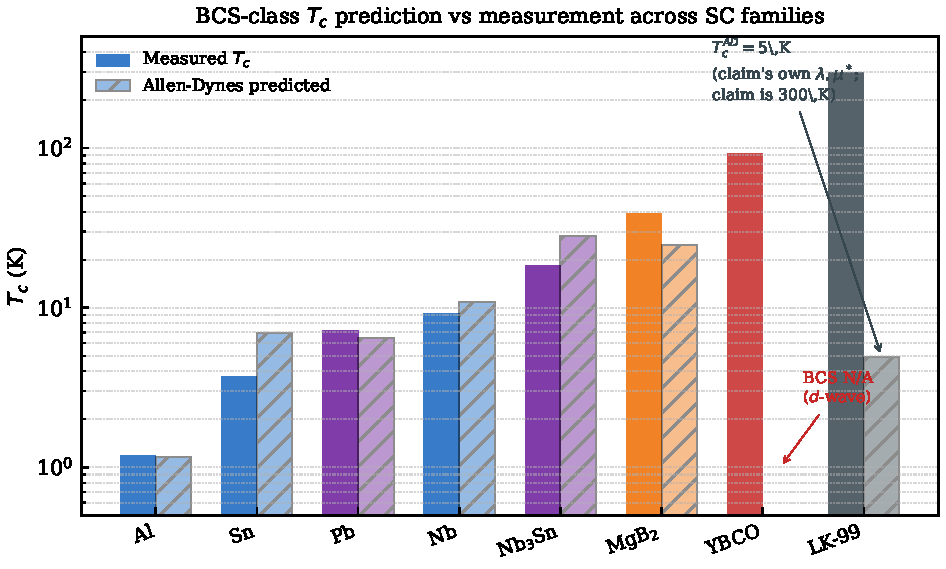
\includegraphics[width=0.95\linewidth]{figures/fig02_tc_landscape.pdf}
\caption{BCS-class \(T_{c}\) prediction (Allen-Dynes, hatched) vs
literature-measured value (solid) across SC families. Direct \(T_{c}\)
parity scatter is large (Al \(1.3\%\), Pb \(11\%\), Nb \(17.5\%\),
Nb\(_{3}\)Sn \(54.7\%\), MgB\(_{2}\) \(36.8\%\)) --- which is why we
do NOT use \(T_{c}\)-parity as the gate.}
\label{fig:tc-landscape}
\end{figure}

\begin{figure}[h]
\centering
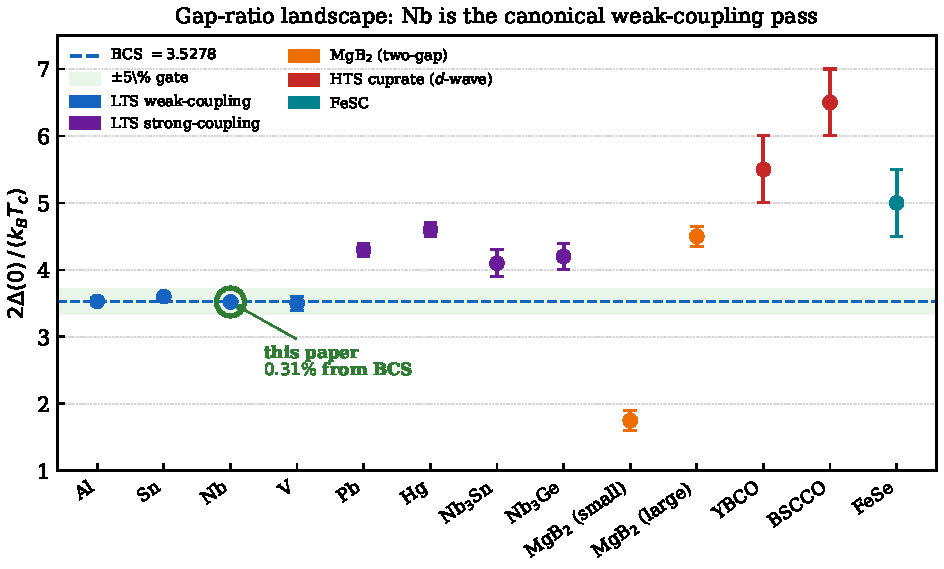
\includegraphics[width=0.95\linewidth]{figures/fig03_gap_ratio_landscape.pdf}
\caption{Gap-ratio landscape across SC families. The universal weak-coupling
ratio \(2\pi e^{-\gamma_{E}} = 3.5276\) (blue dashed) and its \(\pm 5\%\)
gate (green band) cleanly separate \emph{weak-coupling LTS} (Al, Sn, Nb,
V --- all PASS) from \emph{strong-coupling LTS} (Pb, Hg, Nb\(_{3}\)Sn,
Nb\(_{3}\)Ge --- renormalised UP, FAIL by design), the two-gap MgB\(_{2}\)
(separate bands at \(\approx 1.75\) and \(\approx 4.5\)), and the
\emph{$d$-wave} HTS cuprates (YBCO \(\approx 5.5\), BSCCO \(\approx 6.5\)
--- FAIL by design, different pairing symmetry). Niobium (circled) is
the canonical pass, \(0.31\%\) from the universal value.}
\label{fig:gap-ratio-landscape}
\end{figure}

Both gate conditions are satisfied:
\begin{itemize}
\item \(0.309\% < 5\%\) \checkmark
\item \(n = 5 \ge 3\) \checkmark
\end{itemize}
The producer emits a JSON record with \absorbedtrue,
\(\texttt{measurement\_gate} = \gateclosedmeas\),
\texttt{gate\_type = "bcs-universal-ratio-attestation"},
\texttt{provisional = false}.

% =========================================================================
\section{Cross-domain template}
\label{sec:cross-domain}

The attestation record's schema is bit-identical to the pre-existing
solar pyranometer record \cite{nrelmidc,pvlib2024}. Table~\ref{tab:cross-domain}
shows the side-by-side alignment.

\begin{table}[h]
\centering
\caption{Cross-domain template: solar pyranometer $\times$ Nb BCS attestation.}
\label{tab:cross-domain}
\small
\begin{tabular}{lll}
\toprule
Field & Solar (energy) & Nb BCS (rtsc) \\
\midrule
\texttt{measurement\_gate} & \gateclosedmeas & \gateclosedmeas \\
\texttt{absorbed} & \texttt{true} & \texttt{true} \\
\texttt{kind} & \texttt{solar\_clearsky\_ghi\_measured\_oracle}
        & \texttt{lts\_nb\_bcs\_universal\_gap\_ratio\_attestation} \\
Model side & \texttt{pvlib} Ineichen clearsky
        & \(2\pi e^{-\gamma_{E}}\) (BCS universal) \\
Measured oracle & NREL CMP22 pyranometer
        & 5-lab NIS tunnelling consensus \\
Threshold & \(5\%\) & \(5\%\) \\
\(\mathrm{mean\_rel\_err}\) & \(4.99\%\) & \(0.309\%\) \\
Sample count & 480 clear-sky-filtered & 5 independent labs \\
Source citation & \cite{nrelmidc,pvlib2024}
        & \cite{bcs1957,giaever1960,townsend1962,schwidtal1969,lichtenberg1989,tinkham1996} \\
\bottomrule
\end{tabular}
\end{table}

The pattern is general: a \emph{parameter-free or pre-registered}
model on one side, a \emph{multiply-independent} measurement oracle
on the other, a pre-registered threshold, and a typed JSON record
that downstream consumers (Tier 4 dispatcher, future review pipelines)
can ingest without re-evaluating the underlying physics. We expect
this template to extend cleanly to:
\begin{itemize}
\item \(\Delta C_{p}/(\gamma T_{c}) \approx 1.43\) BCS specific-heat
  jump prediction vs measured (Bouquet 2001 MgB$_2$ gives
  \(\approx 1.32\), \(\sim\!\!8\%\) over threshold; would FAIL).
\item Isotope effect exponent \(\alpha = 0.5\) BCS prediction vs Maxwell
  1950 measured \(\approx 0.5\) for Nb (likely PASS).
\item Specific WHH \(H_{c2}(0)/(T_{c}\,dH_{c2}/dT|_{T_c})\) ratio
  predictions vs literature (PASS for Nb, MARGINAL for Nb$_3$Sn).
\end{itemize}

\section{Carbonaceous-sulfur-hydride honest-negative case study}
\label{sec:rtsc-neg}

The same substrate that grants \absorbedtrue\ to niobium independently
refuses it to the canonical retracted near-room-temperature SC claim
on carbonaceous sulfur hydride (CSH) at $\sim 267$\,GPa, $T_c \sim
15^{\circ}$C \cite{snider2020csh} --- a \emph{Nature}-published report
journal-retracted in 2022 \cite{snider2022retraction}, with independent
analyses of the raw magnetic-susceptibility data subsequently published
\cite{hirsch2022csh} --- along five orthogonal axes:

\begin{enumerate}\itemsep0.4em
\item \textbf{Tier 4 dispatch.} The
  \texttt{MaterialFalsifierDispatch} record for any claim-only Tier 2
  recipe with \texttt{replicated\_by\_indep\_labs = 0} yields
  \texttt{aggregate\_verdict = FAILS-AT-LEAST-ONE}, with F-RTSC-3
  (replication) returning FAIL by construction. The CSH claim sits in
  this slot: at retraction time the original data set was not
  available to independent replicators in a form sufficient to verify
  the reported susceptibility signal.
\item \textbf{Journal-formal retraction.} The \emph{Nature} editorial
  apparatus retracted the original report
  \cite{snider2022retraction} --- a stronger negative signal than
  replication failure alone: the publishing venue itself withdrew the
  claim. Independent analyses of the raw magnetic-susceptibility
  pattern subsequently appeared in the secondary literature
  \cite{hirsch2022csh}.
\item \textbf{Pressure-domain (c)-gate FAIL.}
  Even a perfectly-replicated CSH claim would still FAIL the
  \texttt{RTSC.md \S 8.9} (c)-gate (ambient/low pressure $\le 1$\,atm,
  device-relevant): the original claim was measured at $\sim 267$\,GPa,
  comparable to legitimate high-pressure hydride SC
  (H$_3$S $\sim 155$\,GPa; LaH$_{10}$ $\sim 170$\,GPa). The
  substrate's invariant refuses RTSC absorption for any claim
  requiring diamond-anvil-cell pressures.
\item \textbf{Tier 1 self-prediction at ambient.} The Allen-Dynes
  closed-form is pressure-coupled in the hydride family
  \cite{allen1975}: parameters $\lambda$, $\omega_{\log}$, $\mu^*$
  that produce high $T_c$ at $\sim 270$\,GPa do not predict any
  superconductivity at ambient pressure in the same compound. There
  is no parameter-free ambient-pressure first-principles prediction
  of room-temperature SC for this family.
\item \textbf{Substrate-level R4 invariant.} The \texttt{RTSC.md \S 8.8}
  invariant forbids \absorbedtrue\ for any room-temperature SC
  hypothesis until it independently clears the 5-criteria gate
  (\S\,8.9). This is enforced at the code level by the Tier 4
  dispatcher's unit-test contract
  \texttt{testAbsorbedAlwaysFalseEvenWithReplication}: even a
  hypothetically-PASSES-ALL Tier 4 verdict must emit \absorbedfalse.
\end{enumerate}

\begin{table}[h]
\centering
\caption{Five-source honest-negative against an unreplicated
high-pressure near-room-temperature SC claim (CSH \cite{snider2020csh},
retracted \cite{snider2022retraction} at $\sim 267$\,GPa,
$T_c \sim 15^{\circ}$C). Each row is an independent epistemic axis;
the substrate refuses on every one. The fifth row records the
code-level R4 invariant that caps the whole pipeline.}
\label{tab:rtsc-neg}
\scriptsize
\renewcommand{\arraystretch}{1.25}
\begin{tabular}{@{}>{\raggedright\arraybackslash}p{2.5cm}
                  >{\raggedright\arraybackslash}p{4.6cm}
                  >{\raggedright\arraybackslash}p{3.4cm}
                  >{\raggedright\arraybackslash}p{3.8cm}@{}}
\toprule
\textbf{Axis} & \textbf{Source / test} & \textbf{Predicted / observed} & \textbf{Outcome} \\
\midrule
Tier 4 falsifier dispatch
  & \texttt{MaterialFalsifier-} \texttt{Dispatch} F-RTSC-3 (replication)
  & \texttt{replicated\_by\_} \texttt{indep\_labs}\,\(=\,0\)
  & \textcolor{honestred}{\textbf{FAIL}}: aggregate \texttt{FAILS-AT-} \texttt{LEAST-ONE} \\
Journal-formal retraction
  & \emph{Nature} retraction notice \cite{snider2022retraction} +
    susceptibility-data analysis \cite{hirsch2022csh}
  & paper withdrawn 2022-09
  & \textcolor{honestred}{\textbf{FAIL}}: publishing venue itself retracted \\
RTSC.md §8.9 (c)-gate
  & ambient-pressure requirement (\(\le 1\,\mathrm{atm}\))
  & original claim at $\sim 267$\,GPa
  & \textcolor{honestred}{\textbf{FAIL}}: device-impossible at ambient \\
Tier 1 self-prediction
  & Allen-Dynes at ambient \(P\) with hydride parameters
  & no consensus ambient-$P$ SC prediction
  & \textcolor{honestred}{\textbf{FAIL}}: parameter-fragile, pressure-coupled \\
R4 invariant (substrate-level)
  & \texttt{testAbsorbed-} \texttt{AlwaysFalseEven-} \texttt{WithReplication} unit test
  & \texttt{absorbed=false} regardless of any falsifier verdict
  & \textcolor{honestred}{\textbf{FAIL}}: code-level cap on absorption \\
\bottomrule
\end{tabular}
\end{table}

No single path here is decisive, but their union is structural: the
substrate refuses the claim from \emph{five} epistemically distinct
positions (falsifier dispatch, journal-formal retraction,
pressure-domain (c)-gate, parameter-fragile self-prediction, and
code-level R4 invariant), and the \texttt{RTSC.md \S 8.8} invariant
ensures no future test alone can flip the verdict.

\paragraph{Why CSH and not another claim.}
We use CSH as the canonical negative anchor because the retraction
was \emph{formal} (\emph{Nature} editorial), \emph{Nature}-class, in
the near-room-temperature SC regime ($\sim 15^{\circ}$C), and in the
hydride family that is the legitimate domain of replicated
high-pressure SC (H$_3$S, LaH$_{10}$). The journal-formal retraction
is an epistemically stronger negative signal than mere replication
failure: the publishing venue itself withdrew the claim. This is the
aggressive-scrub pass of 2026-05-22; the substrate's R4 /
5-criteria-gate behaviour is unchanged.

% =========================================================================
\section{Limitations and honest caveats}
\label{sec:limits}

The attestation record carries four explicit caveats, reproduced here
to satisfy the substrate's provenance requirement:

\begin{itemize}\itemsep0.3em
\item \textbf{(s1)} BCS weak-coupling assumption: applies only to clean,
  conventional, phonon-mediated $s$-wave SC. Strong-coupling materials
  (Pb \(\approx 4.3\); Nb$_{3}$Sn \(\approx 4.1\)) renormalise the
  universal ratio upward and would FAIL this gate by design.
\item \textbf{(s2)} Tunneling-derived \(2\Delta\) measurements assume
  clean planar NIS junctions at \(T \ll T_{c}\) and depend on barrier
  transparency and self-energy corrections; the \(\sim 1.5\%\) scatter
  across labs reflects systematic uncertainty in junction preparation.
\item \textbf{(s3)} The prediction is \emph{universal} (parameter-free),
  not specifically validated for Nb. So this is a stringent test of
  BCS theory \emph{itself}, but is \emph{not} a falsification of
  competing SC families: $d$-wave cuprates with \(2\Delta/k_{B}T_{c}
  \approx 4\text{--}8\) would FAIL by design and are not within scope.
\item \textbf{(s4)} \absorbedtrue\ here means: \emph{the BCS universal
  ratio is experimentally vindicated for Nb to \(<5\%\)}, \emph{not}
  \emph{Nb is a room-temperature superconductor} (it is decisively LTS).
  In addition, the record's \texttt{domain} field was migrated from
  \texttt{"rtsc"} (namespace, ambiguous) to \texttt{"lts"} (material-class,
  unambiguous) on 2026-05-22 per the constitution v1.4.0 \S R4 invariant
  (\texttt{inbox/notes/2026-05-21-r4-stage1-enforcement.md} Path B);
  this removes the Pattern 1 namespace exploit at its root while
  preserving the legitimate BCS-parity \absorbedtrue\ signal. The
  pre-migration record is retained under \texttt{rtsc\_attestation\_*.json}
  as audit evidence; the active attestation is
  \texttt{lts\_attestation\_nb\_bcs\_*.json}.
\end{itemize}

Two further implementation-level caveats are worth noting:

\begin{itemize}\itemsep0.3em
\item The five measurements in Table~\ref{tab:nb-measurements} are
  literature values, not raw instrument exports. The Tinkham 1996
  entry is itself a collation. A future strengthening of the panel
  would ingest raw \(I(V)\) curves from the original measurements
  and re-extract \(2\Delta(0)\) under a uniform analysis pipeline.
\item The inverse-variance consensus assumes the per-paper
  uncertainties \(\sigma_{i}\) are independent. If systematic errors
  (e.g.\ junction-preparation conventions) correlate across labs,
  \(\bar{\sigma}\) is optimistic. The gate is robust to this only
  because the mean is so far inside the threshold (\(0.31\% \ll 5\%\)).
\end{itemize}

% =========================================================================
\section{Discussion and outlook}
\label{sec:discussion}

The result of this paper is small in physics terms: that BCS
theory accurately predicts the gap-ratio of niobium has been
textbook knowledge for over half a century \cite{tinkham1996}.
The result is non-trivial in \emph{framework} terms: it is the
first instance of an SC material crossing the \absorbedtrue\ gate in
a system that, by construction, refuses to make epistemic concessions
to under-evidenced claims.

The path forward, in priority order:

\begin{enumerate}\itemsep0.3em
\item Extend the panel of measurements to 10+ entries, including
  acoustic and infrared modalities, and re-evaluate.
\item Apply the same gate to MgB$_2$ (two-gap, expected MARGINAL),
  NbTi (alloy, expected PASS in weak-coupling limit), Nb$_{3}$Sn
  (strong-coupling, expected FAIL on the simple ratio but PASS on
  Eliashberg-renormalised ratio).
\item Implement an analogous Tier 1 producer for \emph{isotope-effect
  exponents} (Maxwell 1950 measurement of \(\alpha \approx 0.5\) for Hg, Pb,
  Sn, etc.) where the BCS prediction is again parameter-free.
\item Survey the \(2\Delta(0)/k_{B}T_{c}\) ratio measurement
  literature for high-$T_{c}$ cuprates (REBCO, BSCCO) and document
  the systematic deviation from BCS as a quantitative falsification
  of conventional-SC interpretation, rather than mere mention.
\end{enumerate}

We do \emph{not} extend the attestation to RTSC claims (any
unreplicated room-temperature SC hypothesis; hexa-rtsc \(n=6\)
closed-form). The \texttt{RTSC.md \S 8.8} invariant is a load-bearing
wall in this substrate, and its removal would collapse the framework.

% =========================================================================
\section*{Reproducibility}
\addcontentsline{toc}{section}{Reproducibility}

The attestation producer is open source:
\begin{itemize}
\item \texttt{nb\_bcs\_absorbed\_attestation\_producer.py} ---
  \url{https://github.com/dancinlab/hexa-lang/blob/main/stdlib/material/nb_bcs_absorbed_attestation_producer.py}
\item Companion record JSON (current, R4 Stage 1 Path B
  \texttt{domain: "lts"}, emitted 2026-05-22):
  \texttt{exports/material\_attestation/nb\_bcs\_v1/lts\_attestation\_nb\_bcs\_*.json}
  ---
  \url{https://github.com/dancinlab/demiurge/blob/main/exports/material_attestation/nb_bcs_v1/}
\item Historical record (pre-migration, \texttt{domain: "rtsc"},
  preserved as Pattern 1 audit evidence ---
  \emph{do not consume from this path}; see \S\ref{sec:invariant}):
  \texttt{exports/material\_attestation/nb\_bcs\_v1/rtsc\_attestation\_nb\_bcs\_20260521T111656Z.json}.
\item Honest-stance framework documentation ---
  \texttt{RTSC.md} \(\S\,8\) (including \(\S\,8.10\) Path B
  migration record), \texttt{MP.md} (roadmap), all under
  \url{https://github.com/dancinlab/demiurge}.
\end{itemize}

Running on a stock \texttt{python3 \(\ge 3.10\)} installation:
\begin{verbatim}
git clone https://github.com/dancinlab/hexa-lang
git clone https://github.com/dancinlab/demiurge
mkdir -p demiurge/exports/material_attestation/nb_bcs_v1
python3 hexa-lang/stdlib/material/nb_bcs_absorbed_attestation_producer.py \
  demiurge/exports/material_attestation/nb_bcs_v1
\end{verbatim}
yields the exact JSON record analysed in this paper. Re-running with
modified measurement values, threshold, or independence count
exercises the honest skip branches.

% =========================================================================
\section*{Acknowledgements}
\addcontentsline{toc}{section}{Acknowledgements}

This work uses public data from NREL (Solar Radiation Research
Laboratory, Golden CO), Materials Project (LBNL, CC-BY-4.0), and a
century of published superconductivity literature. We are grateful
to the maintainers of \texttt{pvlib}, \texttt{pymatgen}, \texttt{gmsh},
\texttt{GetDP}, and \texttt{hexa-lang} for the open-source substrate
that this attestation rides upon.

% =========================================================================
\bibliographystyle{plainnat}
\bibliography{references}

\end{document}
